\paragraph{2.6}~{}

根据课上所讲的知识我们知道,对于一个元素排列$p$有
$$Pr(MinHash_p(A) = MinHash_p(B)) = sim(A,B)$$
因此我们可以采用局部敏感度哈希的方法进行统计,从而计算出相似度较高听众对,具体步骤如下。
\begin{enumerate}
\item 对于每个人构建一个集合$A_i$表示第$i$个人喜爱的歌曲的集合,
\item 使用课上所讲的MinHash,将歌曲序号进行随机排列,对于每个人$i$找出$A_i$中出现在排列中最靠前的歌曲序号,作为此次MinHash的值,这样我们会得到每个人此次的minhash取值。
\item 重复第2步$k$次,可以得到一个$k * n$的哈希签名矩阵,
\item 对哈希签名矩阵行进行分割,分割成$B$个brand(一个brand有$r = k/B$行)。
\item 对于每一个brand,我们将$n$个人的在当前brand中的$r \times 1$的子矩阵进行再次哈希,按照哈希值将其放进桶内,此时我们保证桶数量尽可能多。
\item 如果有同一个brand的不同两列哈希之后映射在同一个桶内,那么认为这两列对应的用户是相似的。
\end{enumerate}
我们对该算法进行分析,设两个用户的喜爱歌曲相似度为$s$,那么在所有brand中至少存在一个brand使得二者的哈希值相同的概率为
$$Pr = 1-(1-s^r)^B, s \in [0,1]$$

当参数固定时,我们可以将图像画出来
\begin{figure}[H]
    \centering
    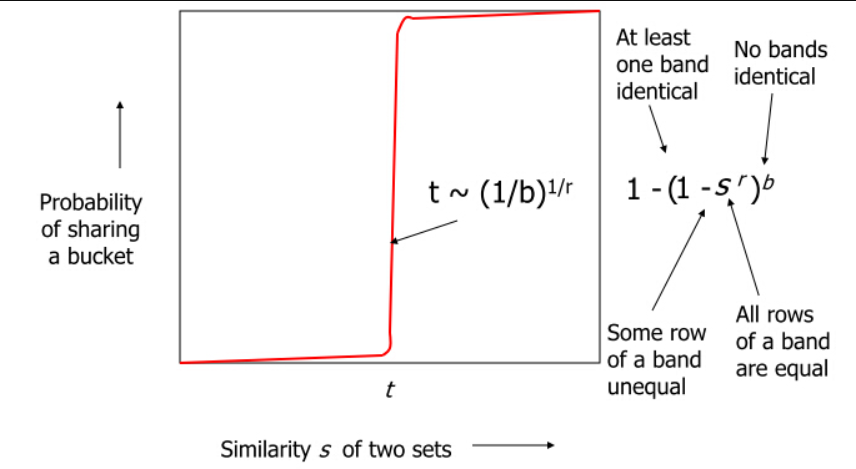
\includegraphics[width=5in]{img/img1.png}
    \caption{$s$与$Pr$关系图}
\end{figure}
由图像我们可知,当两个用户喜爱歌曲的相似度超过阈值t时,会有极大的概率使得至少一个brand内两个用户对应的hash值相同。
因此我们可以认为同一个桶内的元素对应的用户喜爱歌曲的相似度是超过阈值$t$的。

而我们可以通过参数的设置来设置阈值:
$$S(t) = (\frac{1}{B})^{\frac{1}{r}}$$

